\documentclass{article}

\usepackage{graphicx}
\usepackage{caption}
\usepackage{rotating}
\usepackage{float}
\usepackage[margin=0.8in]{geometry}
\usepackage[section]{placeins}
\usepackage[hidelinks]{hyperref}
\usepackage{sectsty}
\sectionfont{\clearpage}
\usepackage{csquotes}
\MakeOuterQuote{"}

\setlength{\parskip}{0.3em}
\usepackage{xcolor}
\usepackage{listings}
\lstset{
	language=Verilog,
	frame=single,
	basicstyle=\small,
	keywordstyle=\color{blue}\small,
	stringstyle=\color{Maroon}\small,
	commentstyle=\color{OliveGreen}\small,
	breaklines=true,
	postbreak=\raisebox{0ex}[0ex][0ex]{\ensuremath{\color{red}\hookrightarrow\space}}
}

\title{FPGABoy Documentation}
\author{Luke Wren}

\begin{document}

\pagenumbering{gobble}
\maketitle
\tableofcontents
\newpage
\pagenumbering{arabic}

\section{Introduction}

FPGABoy is an open source portable games console, designed from scratch. It is also...
\begin{itemize}
\item An open source PCB layout
\item Designed with KiCAD open source PCB editor
\item An open source CPU, graphics and bus architecture
\item Based on the RISC-V open source instruction set
\item Synthesised, placed and routed with iCEStorm open source FPGA toolchain
\item It's open source
\end{itemize}

\begin{displayquote}
\textit{If you say open source one more time I'm gonna nut instantly} - Oscar Wilde
\end{displayquote}

\subsection{Digital Design}

\begin{figure}[!htb]
\caption{System-level architecture}
\label{diagram:system_arch}
\centering
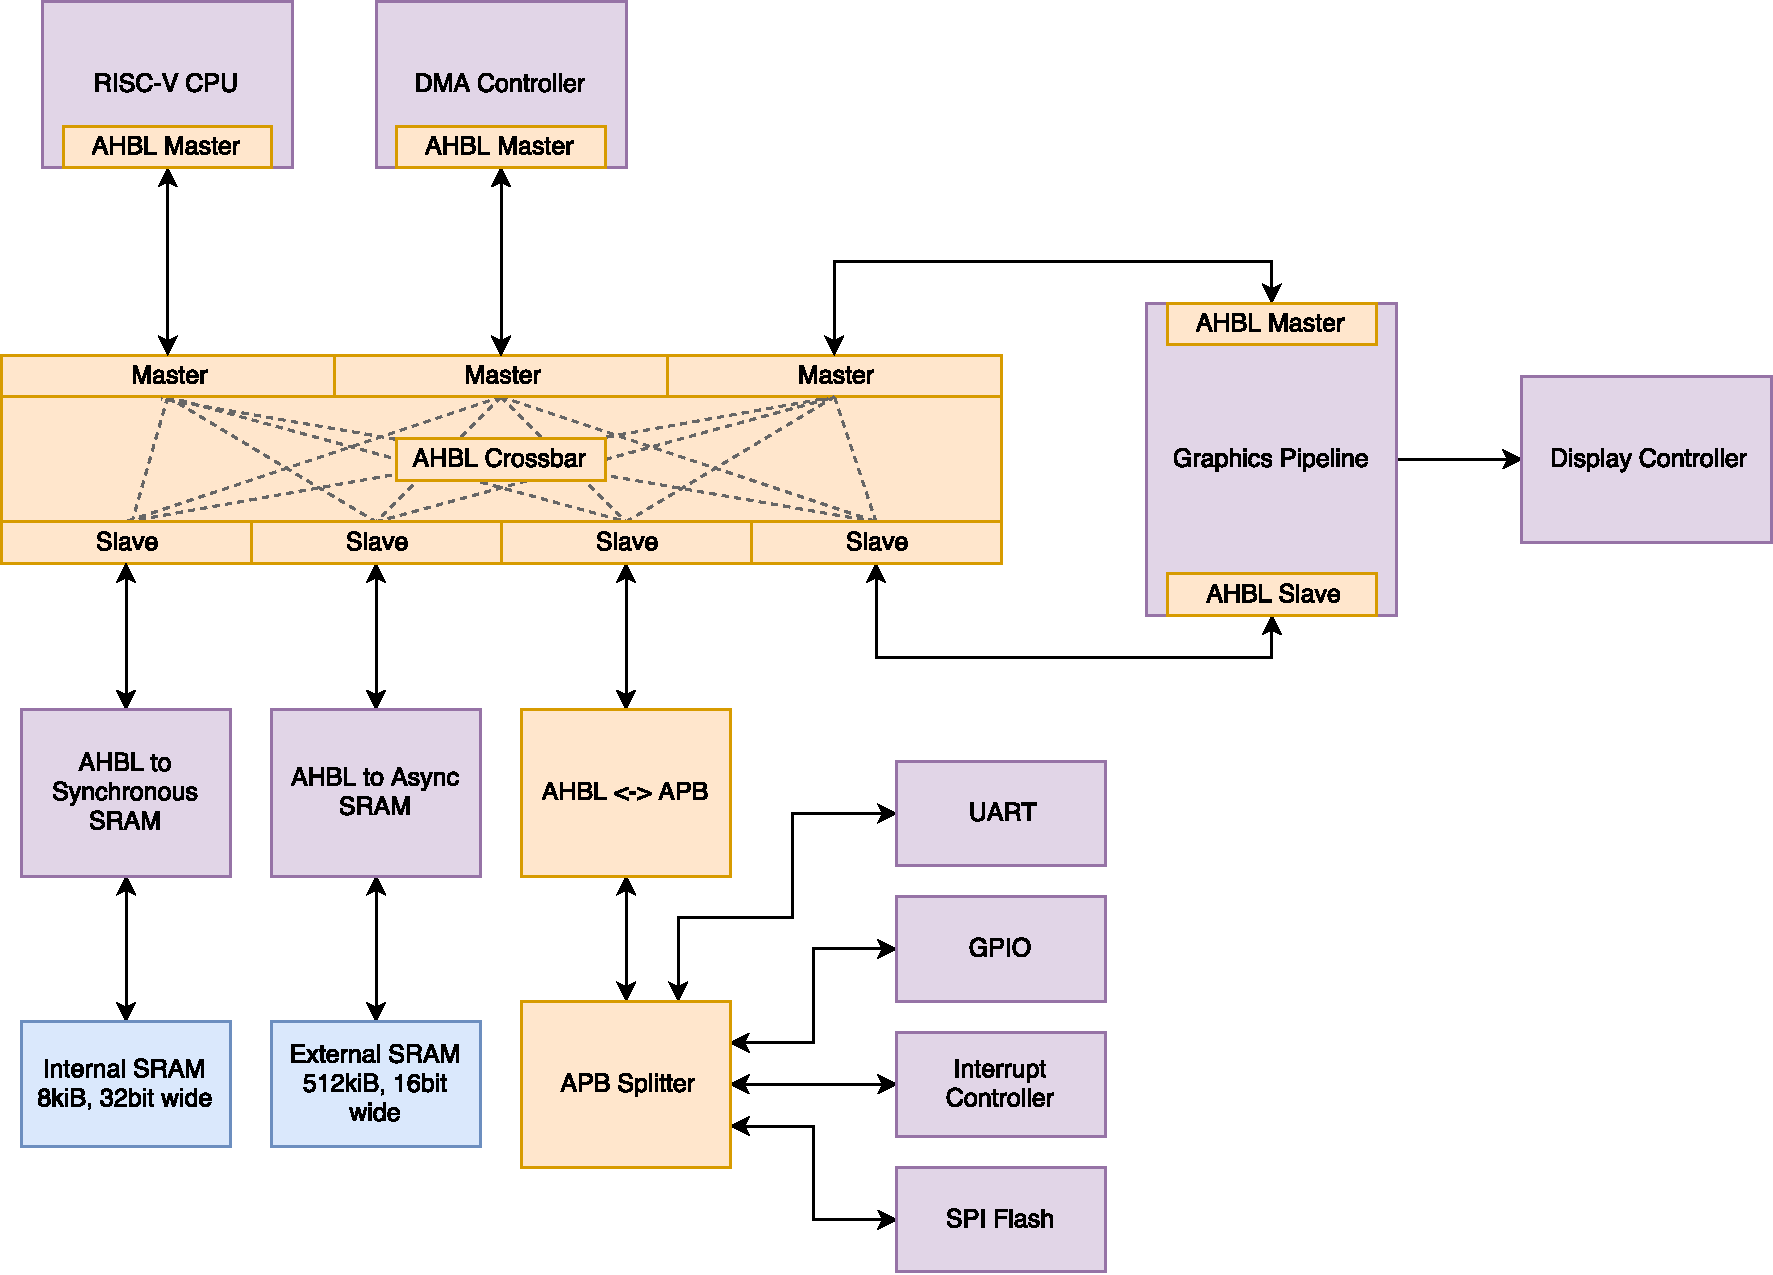
\includegraphics[width=0.7\textwidth]{diagrams/system_arch.pdf}
\end{figure}

The heart of the design is a Lattice iCE40-HX8k FPGA, containing 7680 LUT4s and flipflops. The logic was designed in synthesisable Verilog, with no dependencies on FPGA vendor IP (or anything else); the contents of this GitHub repository could be taped out onto a chip. This includes:

\begin{itemize}
\item RV32IC-compatible 32-bit CPU design
	\begin{itemize}
	\item RISC-V instruction set
	\item 32I: base integer ISA profile
	\item C: compressed instruction extension, for higher code density
	\item Vectored interrupts (save/restore of PC, RA only)
	\item 5-stage pipeline, similar to textbook RISC
	\item Single AHB-lite master port
	\end{itemize}
\item Graphics pipeline
	\begin{itemize}
	\item Don't expect much, it's about as powerful as a Gameboy Advance
	\item Includes some MODE7-like functionality which allows drawing perspective-mapped textured planes, by providing per-scanline affine texture transformation. Think MarioKart
	\end{itemize}
\item AMBA 3 AHB-lite compatible multi-master busfabric
\item Peripherals:
	\begin{itemize}
	\item DMA master
	\item External asynchronous SRAM controller (GS74116 or similar)
	\item Display controller (ILI9341)
	\item SPI flash controller with direct memory-mapped access
	\item GPIO (bitbanging, peripheral muxing)
	\item Interrupt controller
	\item UART
	\item PWM
	\item Basic audio: voices + samples, noise-shaped PWM output
	\end{itemize}
\end{itemize}

Some attempt is made in this document to describe the operation of these blocks, but if you are looking for nitty-gritty detail, the best documentation is the files ending with \texttt{.v}.

That a free synthesis tool can cram all this logic into one of the cheapest FPGAs on the market is tremendously impressive. Hopefully we will one day have a situation similar to software compilers, where free tools such as GCC are industry standards.

\subsection{PCB}

The board is a 4-layer stackup:

\begin{enumerate}
\item Signal + GND Fill
\item GND plane
\item Power planes
\item Signal + GND Fill
\end{enumerate}

It is intended to be suitable for low-cost PCB prototyping services such as iTead. Board dimensions are 50mm $\times$ 50mm, which fits into the cheapest size category on iTead. For the most part, it sticks to the following minimum specifications:

\begin{itemize}
\item Track width 0.15mm
\item Copper-copper clearance 0.15mm
\item Soldermask-copper clearance 0.1mm
\item Soldermask width 0.1mm
\item Via drill 0.3mm
\item Annular ring 0.15mm (i.e. via diameter 0.6mm)
\end{itemize}

The only exception is some 0.5mm vias underneath the BGA. Strictly this is out of specification for iTead, but they claim to have a 90 $\mu$m drill registration, so we'll see how it goes.

The iCE40-HX8k FPGA is packaged in a 256-pin 0.8mm BGA, which \textit{can be} reflowed by a hobbyist with a hot air gun or a frying pan (best to choose a HASL finish so that contacts are pretinned). The 132-pin 0.5mm BGA has sufficient IO for our needs, but iTead does not manufacture at the tolerance required for such a fine pitch.


\subsection{Licensing}

The Verilog source to this project has no dependencies, and is distributed under the DWTFPL version 3. This is a \textit{very} permissive open-source licence, and its text is included in full at the top of the source files. This license is very similar to the original DWTFPL, which more readers may be familiar with, but has an added indemnification clause.

This license is also known by its more formal name, as the "Do What The Fuck You Want To And Don't Blame Us Public License".

\section{CPU Architecture}

ReVive is a 32-bit processor based on the RISC-V instruction set architecture. It yearns for the glory days of games programming, when NULL pointers were just pointers to the start of ROM, and programmers were real programmers who wrote their \textit{own} polygon rasterisers, dammit. Targeting a small FPGA, ReVive sits mostly in the embedded design space -- RV32IC is an austere instruction set. It does make some concessions to performance, such as a 5-stage pipeline with full bypass.

Figure \ref{diagram:cpu_pipeline} shows a simplified block diagram of the core. Not shown is:
\begin{itemize}
\item The full and specific contents of the pipeline registers
\item Interrupt entry/exit hardware
\item The ready/valid handshakes on pipe stages which allow them to NOP later stages, and stall prior ones
\item Stall-generation logic
\item Pipeline flushing signals for branch mispredict
\item Hardware for supporting unaligned loads/stores (carried out as multiple bus cycles)
\end{itemize}

Overall this is a standard RISC-style pipeline. The tall blue boxes represent the registers at the boundaries of two pipe stages. The nomenclature used in the diagram is:

\begin{itemize}
\item \texttt{F}: fetch
\item \texttt{D}: decode
\item \texttt{X}: execute
\item \texttt{M}: memory access (load/store)
\item \texttt{W}: register writeback, fetch address generation
\end{itemize}

Branches are speculated, according to the static prediction scheme described in the RV ISA manual:

\begin{itemize}
\item Backward branches predicted taken; hopefully, loops run at least twice on average.
\item Forward branches predicted not taken; the ISA manual advises compilers should put more-likely code on this path.
\end{itemize}

The processor has one AHB-lite busmaster, arbitrating internally between instruction fetch and data load/store. If \texttt{F} hits the instruction cache (which has room for 16 compressed instructions, 8 words), no AHB request is issued. The ideal use case for \texttt{ICACHE} is a function like \texttt{memcpy}: the inner loop executes from cache only, leaving the busmaster free for loads and stores. The small size allows it to fit into the pipeline in an interesting place, without imbalance.

\begin{displayquote}
\textit{It's not the size, mate, it's how you use it.} - Austin Powers, Goldmember
\end{displayquote}


\newpage

\begin{center}
	\begin{sideways}
		\begin{minipage}{\textheight}
			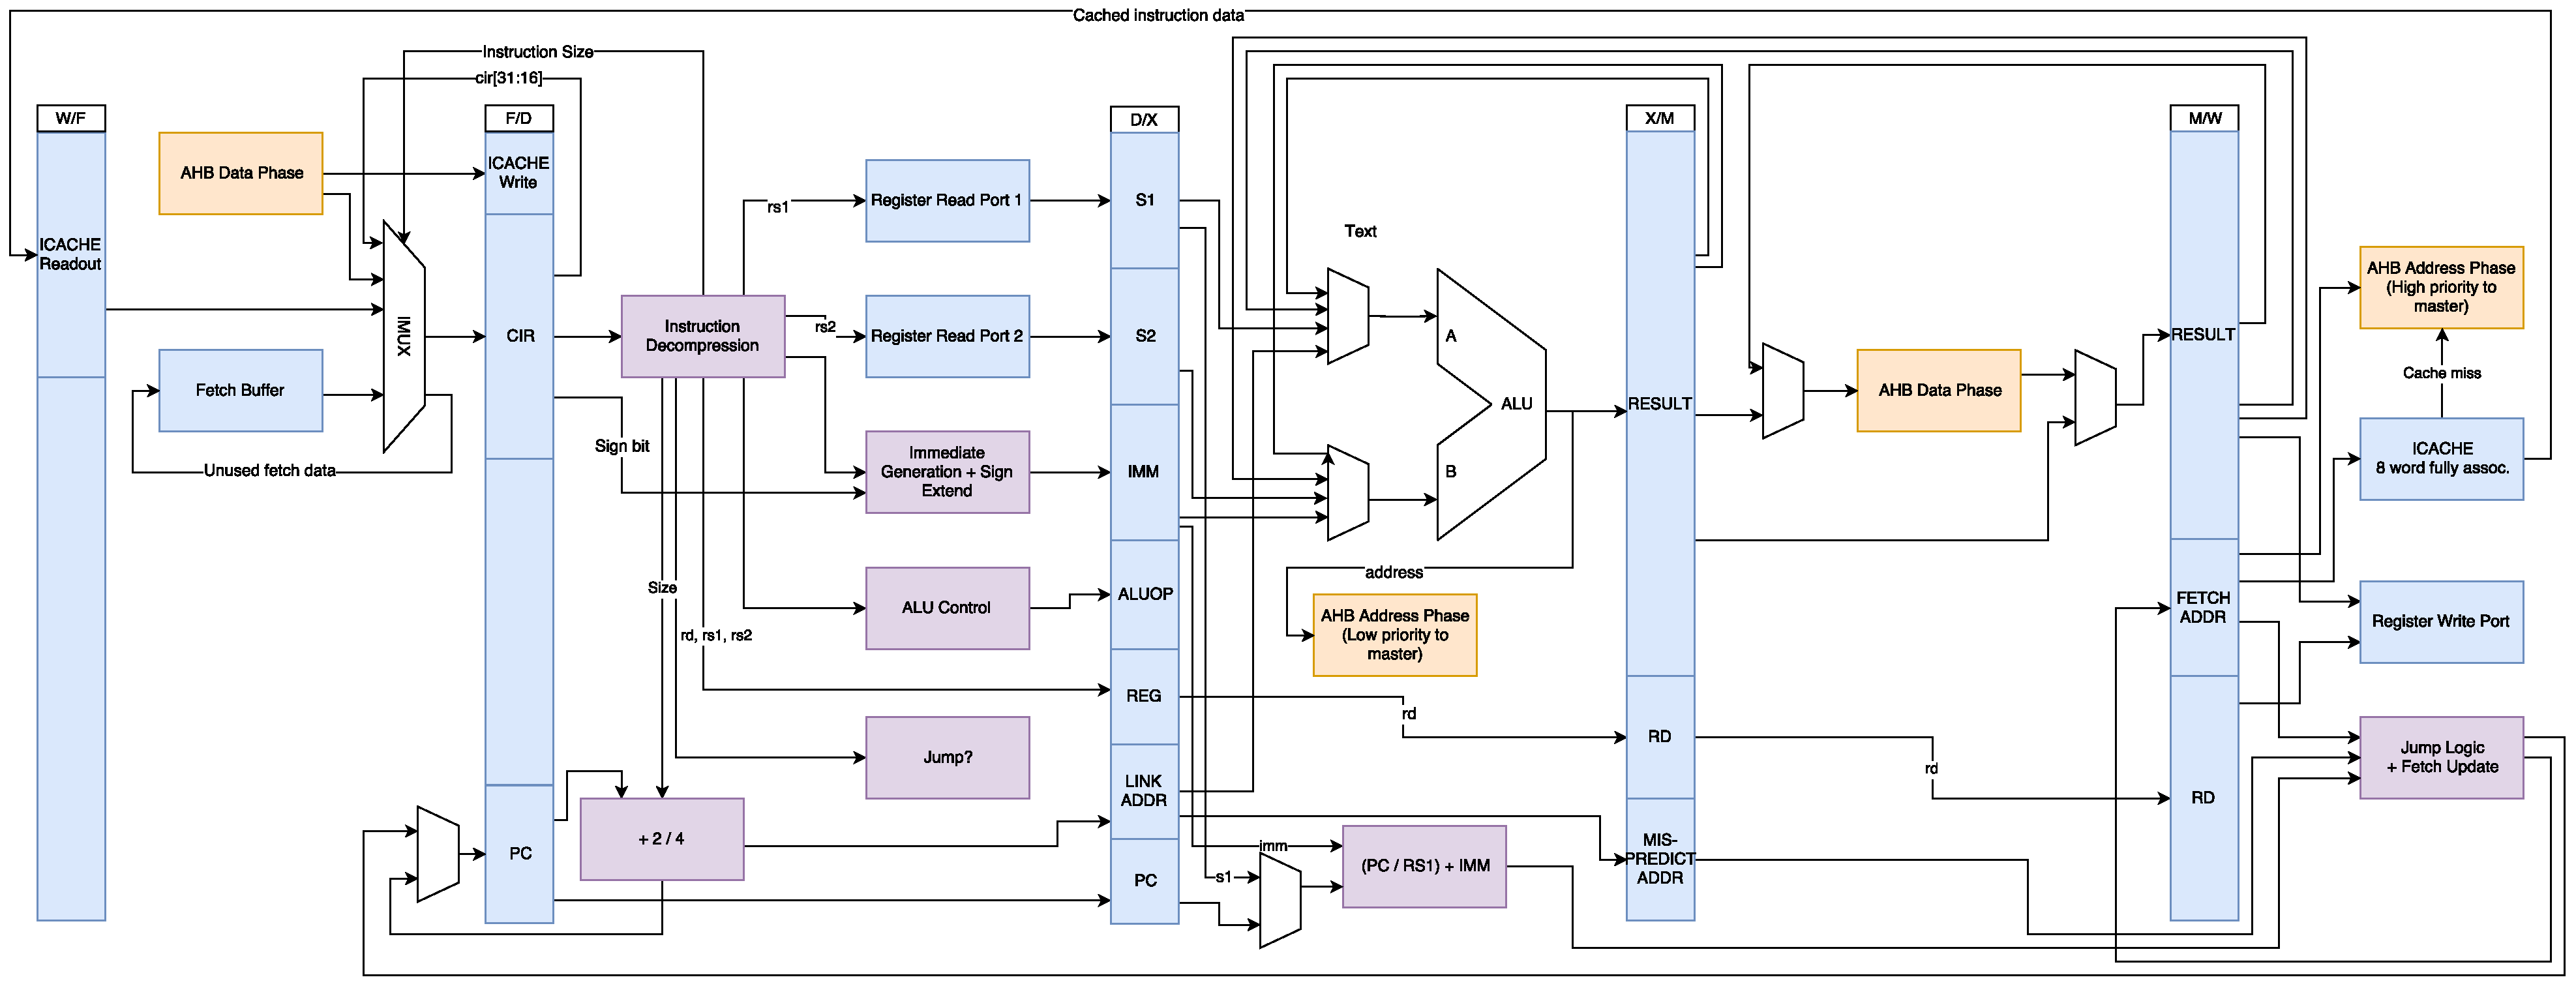
\includegraphics[width=\textheight]{diagrams/cpu_full.pdf}
			\captionof{figure}{ReVive architectural block diagram}
			\label{diagram:cpu_pipeline}
		\end{minipage}
	\end{sideways}
\end{center}

\newpage

\subsection{Fetch Logic}

\texttt{F} always provides \texttt{D} with 32 bits of fresh instruction data, in the canonical RISC-V order (halfword-wise little-endian). There are four sources:

\begin{itemize}
\item AHB busmaster with access to system memory map
\item \texttt{ICACHE}. A small, fully-associative cache with random eviction
\item An \texttt{F}-local buffer containing up to 32 bits of fetched, unused instruction data
\item The second halfword of the current instruction register of \texttt{D}, in the case that \texttt{D} found the last instruction to be 16-bit
\end{itemize}

The pipeline register \texttt{F} writes to, containing the 32 fresh instruction bits, is referred to internally as current instruction register or \texttt{CIR}.

AHB instructions fetches are \textit{always} word-sized, word-aligned. Internal buffering and muxes take care of building unaligned instruction bundles from this aligned data stream.

\subsubsection{The Fetch Buffer}
\label{section:fetch_buffer}

Upon request, \texttt{F} can receive 32 bits of instruction data in a given cycle, via AHB or ICACHE. This request has a one-cycle latency. In the same cycle, \texttt{F} will consume 16 or 32 bits to refill \texttt{CIR}, based on the size of the instruction currently being decoded (which can quickly be ascertained by inspecting the two least-significant bits).

The combination of request latency, and sometimes receiving more data than we need, suggests a need for buffering in the fetch stage. But how much? And what is the optimal rule for deciding whether to make a fetch request? Looking at the information we have to hand in a given cycle:

\begin{itemize}
	\item $b_n$, the current buffer level in halfwords
	\item $i_n$, the size of the instruction currently being decoded
	\item $f_{n-1}$, whether we made a fetch request on the previous cycle
\end{itemize}

we can come up with the following update rule for the buffer level on the next cycle:

\[ b_{n+1} = b_n - i_n + 2f_{n-1} \]

And our task is to choose $f_n$ such that $b_n$ stays between 0 and the smallest possible positive integer. We can clearly rule out 0 as a possiblity for the buffer size, and can also rule out 1, since a fetch is required if $b_{n+1} = 1$ to avoid underflow if the next instruction is 32-bit, and this fetch will cause overflow if the next instruction is 16-bit.

However, 2 halfwords works, if we apply the rule that we request a fetch on cycle $n$ if $b_{n+1} < 2$: if $b_{n+1} = 2$,  $b_{n+2}$ would then be 0 or 1, and any other value for $b_{n+1}$ could not cause overflow since buffer level cannot increase by more than 1 per cycle. Since 2 is a lower bound, it is the optimal size for the buffer, and this rule is also optimal.

At start of day, we initialise the \texttt{CIR} and the fetch buffer with a 32-bit \texttt{nop} each, the buffer level to 2, and $f_{n-1}$ to zero (since there \textit{was} no previous cycle to fetch on!). According to our rule, \texttt{F} will request a fetch on the first cycle (which will be from the reset vector), kicking off an AHB address phase; \texttt{D} will decode a \texttt{nop} on this cycle, the \texttt{CIR} will be refilled with the \texttt{nop} from the buffer, and the buffer level will go to zero. On the next cycle, \texttt{D} will decode the second \texttt{nop}, and \texttt{CIR} will be refilled again, this time with the instruction data from AHB. The buffer level will remain at 0. We have reached our execution steady state, from reset, without having any special purpose logic to handle reset. We have just chosen our flipflop reset values carefully.

There is one extra case where we may expect to need more than two halfwords of buffering: what happens if an AHB dataphase completes whilst \texttt{D} is stalled? We would have a surplus of data, and would either have to drop some fetch data and restart that fetch (at a cost of 2 cycles), or would require up to an extra word of buffering. The resolution is to examine the cases where \texttt{D} is actually stalled: either this is due to a low \texttt{hready} -- in which case \textit{by definition} this is not the last cycle of a data phase -- or we are stalled on a RAW hazard between \texttt{X} and \texttt{M}. This will only happen if the instruction in \texttt{M} is a load. On the previous cycle, this load was in \texttt{X}, where it would have won arbitration over the code fetch address phase -- hence, there cannot be data arriving in \texttt{F} on the current cycle, and no extra buffering is required.

\subsubsection{Sequential Code}

In sequential code, the \texttt{ICACHE} will be queried every cycle (unless the fetch buffer is full), during \texttt{W}, as to whether it has the next aligned word. We are able to guarantee that all AHB and \texttt{ICACHE} accesses are word aligned due to the operation of the fetch buffer in \texttt{F}.

The query response is combinatorial, and is used to decide whether to assert an AHB access during the address phase. Successful queries will result in cached read data appearing on the next clock edge, for use by \texttt{F}.

\texttt{F} is concurrent with the AHB data phase, except for a small muxing layer at the end which assembles the instruction word from AHB data, buffered data and cached data.

Following an unsuccessful \texttt{ICACHE} query, \texttt{F} will write the AHB data into the cache, evicting one word of its present contents. \textit{The same address must not appear more than once in the cache}, as the query logic is based on a non-priority sum of product encoder.


\subsubsection{Jumps}
\label{section:jumps}

When jumping or taking a branch, \texttt{F} invalidates its fetch buffer, and ignores present \texttt{CIR} contents. Aligned jumps are otherwise no different from sequential code: \texttt{ICACHE} is queried with the jump address, and AHB supplies the data if \texttt{ICACHE} does not have it.

Unaligned jumps (i.e., halfword-aligned but not word-aligned) are more painful, as we may need to perform two accesses to fetch the required data:

\begin{enumerate}
	\item \texttt{W} queries the cache with the address of the word containing the first instruction halfword
	\begin{itemize}
		\item If we hit \texttt{ICACHE}, we issue an AHB read to fetch the \textit{second} word in parallel with reading out from the cache
		\item If we miss, we issue an AHB read to fetch the first word from system memory.
	\end{itemize}
	\item On the next cycle, we have either 32 or 64 bits of fetch data available to \texttt{F}, depending on cache hit/miss
	\begin{itemize}
		\item The first halfword is useless
		\item If we have only 32 bits, then we put the second halfword into \texttt{CIR}, and assert a flag to inform \texttt{D} that only this halfword is valid
		\item If we have 64 bits, we forward the middle two halfwords to \texttt{CIR}, and stash the final halfword in the fetch buffer. Normal execution resumes.
	\end{itemize}
	\item If \texttt{CIR} was half-valid:
		\begin{itemize}
			\item \texttt{D} reports instruction was 16-bit: we got away with it.
			\item \texttt{D} reports 32-bit instruction: \texttt{D} stalls, \texttt{F} sends a full \texttt{CIR} based on new fetch data from this cycle.
		\end{itemize}
\end{enumerate}

\subsubsection{ICACHE Writeback}

The encoder logic used in the cache lookup does not give correct output if a tag appears multiple times in the cache (however, it is smaller/faster as a result). There is a behaviour pattern that could put \texttt{ICACHE} into an invalid state if we fetched from the same address on consecutive cycles:

\begin{enumerate}
	\item Miss on first cycle; \texttt{W} performs an AHB address phase.
	\item Writeback data not visible until end of this cycle; \texttt{W} performs duplicate AHB address phase.
	\item One copy of data has been written to \texttt{ICACHE}; another write is in progress. \texttt{W} hits \texttt{ICACHE} on this cycle, so no AHB address phase.
	\item The second write has put \texttt{ICACHE} into an invalid state; fetch behaviour is undefined from this point.
\end{enumerate}

Extreme care is required to avoid this pitfall. This sequence does not occur during normal execution: sequential code fetches are to incrementing addresses, and jumps (including jump-to-self) have a penalty cycle, which prevents the double-write behaviour. However, stalls must be treated carefully.

\subsubsection{Program Counter}

ReVive does \textit{not} use the program counter (\texttt{PC}) for code fetching, during sequential execution. It is used exclusively for the first fetch cycle of jumps/branches, the link value in \texttt{JAL(R)}, and branch mispredict recovery.

\texttt{W} fetches instruction data from consecutive word-aligned addresses, as described in section \ref{section:jumps}. \texttt{F} has \textit{flow} control, and can inhibit \texttt{W}'s address phase on any given cycle; \texttt{W} never requires the value of \texttt{PC} during normal operation. However, during non-sequential execution, it does require a \texttt{PC} value. Bits [31:2] are used to set the new fetch address, and bit 1 is used to determine whether the first instruction is aligned or unaligned with the fetch. The difference is outlined in section \ref{section:jumps}: essentially, on an unaligned jump, the first 16 bits of the fetch data are ignored, and the hardware scrabbles to put together a valid instruction.

The true \texttt{PC} lives in \texttt{D}, where it is incremented by 2 or 4 each cycle, depending on the size of the instruction currently in the \texttt{CIR}. The current values of \texttt{PC} and \texttt{PC\_next} both travel into the \texttt{D/X} pipe register, where they are used for relative jump target calculation, and mispredict recovery (later down the pipe, in \texttt{M}), respectively. It may be surprising that we need both of these values, rather than just looking one stage back in the pipeline to get the "next" value. We need to buffer both values because \texttt{D}'s \texttt{PC} is clobbered when we take a branch, so we can not use it for mispredict recovery.

\subsubsection{Load/Store, Fetch Arbitration}

The single AHB master port asserts transactions from two sources: the fetch unit, whose address phase is in \texttt{W}, and the load/store unit, whose address phase is in \texttt{X}. The arbitration rule is that load/store wins over fetch, \textit{unless} a jump is triggered by \texttt{M}, in which case fetch wins. (This includes mispredict recoveries).

The rationale for the main rule is that arbitrating either way can cause a bubble to appear in the pipeline, either after \texttt{F} or after \texttt{X}. However:

\begin{itemize}
	\item \texttt{F} may still be able to cover the next fetch cycle with its buffer contents, in which case we don't lose any cycles
	\item Stalling \texttt{X} on AHB contention also stalls previous stages, including \texttt{F}; \texttt{F} needs to buffer the AHB transaction which will occur during this stall.
\end{itemize}

The rationale for the exception is that a late jump/branch should invalidate newer instructions in the pipeline, so it doesn't make sense for \texttt{X} to be given preferential access to a resource in this case, let alone be allowed to have side effects on system memory.

On cycles where code fetch loses arbitration, \texttt{F} does \textit{not} set its flag which indicates an AHB address phase took place ($f_n \to f_{n-1}$). On the next cycle, \texttt{F} looks at next buffer level, $b_{n+1}$ (see section \ref{section:fetch_buffer}), and inserts a pipe bubble if this value is negative.

Note that this creates some oddities in instruction flows for long strings of loads/stores: the load/store unit will remain active, blocking the fetch port, until the bubbles created by \texttt{F} reach it. The fetch unit will then win until the bubbles have elapsed. This shouldn't affect performance (the busmaster is always occupied, so memory is the bottleneck), it's just a bit weird.


\subsection{Jumps and Branches}

Due to the pipelined nature of AHB, we are unable to jump or to take branches in fewer than 2 cycles (without some fairly sophisticated prediction):

\begin{itemize}
\item Cycle 0: AHB address phase to fetch jump/branch instruction
\item Cycle 1: AHB data phase for fetch of jump/branch. Next instruction is in address phase concurrently.
\item Cycle 2: Jump/branch instruction is now available to \texttt{D}
	\begin{itemize}
		\item (Quickly) use to control the new address phase
		\item The immediately following instruction is already in data phase
	\end{itemize}
\item Cycle 3: data phase for jump target instruction
\end{itemize}


We've paid one penalty cycle in the pipeline (cycle 2), and also made one wasted code fetch.

Jumps are physically taken in \texttt{W}, directly in front of the fetch address generator. There are two reasons to jump:

\begin{itemize}
	\item Inspecting the \texttt{CIR} in \texttt{F/D} pipe register (\texttt{JAL}, speculated taken branches)
	\item Inspecting \texttt{X/M} pipe register (\texttt{JALR}, branch mispredict)
\end{itemize}

\texttt{JALR} (indirect jump) is taken later because it uses the register file and the ALU to compute its target.

If both of these sources attempt to jump in the same cycle, \texttt{X/M} takes priority, since it is executing an older instruction. In both cases, the part of the pipeline in the hazard shadow is invalidated; i.e., \texttt{W} $\to$ \texttt{F}, or \texttt{W} $\to$ \texttt{X}. Invalidation is performed by clobbering the pipeline control signals in such a way that these instructions will have no side effects.

The branch prediction scheme is static: take backward branches, and do not take forward branches. The cycle costs are as follows:

\begin{center}
\begin{tabular}{l c}
\hline
Jump Type & Cycles (Execution + Penalty) \\
\hline
Direct jump & 2 \\
Predicted, non-taken branch & 1 \\
Predicted, taken branch (same as jump) & 2 \\
Indirect jump & 4 \\
Branch mispredict & 4 \\
\hline
\end{tabular}
\end{center}

Upon jumping, we need some mechanism to invalidate parts of the pipeline: this is described in section \ref{section:stalling_flushing}.

\subsection{Operand Bypass}

ReVive provides a multiplexed operand bypass (forwarding) network. Register writes by a given instruction must always be visible to later instructions, even \textit{before} the first instruction reaches the register writeback stage. This is shown as multiplexers on the ALU inputs in figure \ref{diagram:cpu_pipeline}.

This removes, or at least shortens, read-after-write data hazards in the pipeline, and allows us to approach one clock-per-instruction execution rates. Without bypassing, only one instruction could be present in $\left\{ \texttt{D}, \texttt{X}, \texttt{M}, \texttt{W} \right\}$ at a time, giving a CPI of 4.

The following bypasses are available: (notation: pipe register $\to$ pipestage logic)

\begin{itemize}
	\item \texttt{X/M} $\to$ \texttt{X}
	\item \texttt{M/W} $\to$ \texttt{X}
	\item \texttt{M/W} $\to$ \texttt{M}
	\item \texttt{M/W} $\to$ \texttt{D} (internal bypass in register file for write port $\to$ read port)
\end{itemize}

To control the bypassing, some of the register specifiers from \texttt{CIR} are passed down the pipeline alongside the data. \texttt{rs1, rs2, rd} (operand sources and destination) are passed down as far as \texttt{X}. \texttt{rs2, rd} make it to \texttt{M}, and \texttt{rd} makes it to \texttt{W}.

These serve the following purposes:

\begin{itemize}
	\item \texttt{rd} is needed in \texttt{W} anyway, for performing the actual writeback
	\item \texttt{X} looks at the two operand source registers it depends on, and then glances across at the \texttt{rd}s awaiting writes in \texttt{M} (i.e. its own output) and \texttt{W} (i.e. a load output, or an \texttt{X} output one cycle prior).
	\item \texttt{M} Looks at the \texttt{src} register for a store (encoded in the \texttt{rd2} specifier field), and will look at the pending register write in \texttt{W}, which will be either a load result or a prior \texttt{X} result.
\end{itemize}

Architecturally, it may be preferable to perform these bypasses earlier, since RISC-V makes operand decode very simple, with fixed bitfield position for rd1, rd2. That is, put the muxes between the register file and the \texttt{D/X} pipe register, and move the taps to make the hazards work. However, we want the register file to support BRAM inference on iCE40 FPGAs, as we otherwise use about 15\% of the flops on the device just to implement the registers. iCE40s have a synchronous BRAM read port, so the muxes end up after the "pipe register", i.e. the BRAM output registers.

The upshot is:

\begin{itemize}
	\item Back-to-back ALU operations execute at 1 CPI
	\item Loads execute at 2 CPI if they are immediately required by the ALU. 1 CPI otherwise.
	\item Stores execute at 1 CPI
	\item In a load-store pair, the load takes only one cycle, since the \texttt{M} stage has cyclic forwarding
\end{itemize}

\subsection{Pipeline Stalling and Flushing}
\label{section:stalling_flushing}

Our terminology: stalling means a pipeline stage, along with prior stages, does not advance its state until some blocking condition has cleared. Flushing is when in-flight instructions in some stages are replaced with NOPs, and their results are discarded.

All stages stall on HREADY low, no matter which internal master instigated the current data phase. TODO: this is non-optimal. For example, if code fetch is stalled, stages \texttt{D,X,M} could still proceed. This would save one cycle in the case that \texttt{X} is stalled in a RAW hazard on \texttt{M}. We may save \textit{some} cycles on a jump/branch which would cause the current fetch data phase to be ignored; however, AHB does not allow us to assert a new address whilst the current address phase is in progress, so the whole pipe would still stall on the code fetch once the jump/branch is ready to be asserted. For now it seems best to proceed with the simple option.

Besides HREADY low, each stage may stall for the following reasons:

\begin{itemize}
	\item \texttt{F}:
	\begin{itemize}
		\item Fetch buffer underflow (after losing busmaster arbitration)
		\item  Stall in \texttt{X}
	\end{itemize}
	\item \texttt{D}: stall in \texttt{X}
	\item \texttt{X}: RAW hazard on \texttt{M}
	\item \texttt{M}: only on HREADY
	\item \texttt{W}:
	\begin{itemize}
		\item Writeback: only on HREADY
		\item PC generation: stalls when \texttt{X} is stalled.
	\end{itemize}
\end{itemize}

Pipeline bubbles are inserted into a pipe register by the rightmost stage in the stall chain. This stage creates the bubble by zeroing out the destination register field, memory op field, and any other fields which cause side effects. Under the above stall policy, only \texttt{X} will need to create bubbles: this ends up a single bubble, on an \texttt{M} $\to$ \texttt{X} RAW hazard.

There are two cases where we must flush:

\begin{itemize}
	\item Branch/jump taken from \texttt{D}; must flush \texttt{F}.
	\item Jump/mispredict taken from \texttt{M}; must flush \texttt{F}, \texttt{D}, \texttt{X}
\end{itemize}

And the flushing mechanisms for each stage are as follows:
\begin{itemize}
	\item \texttt{F}: Write a flag in \texttt{F/D} which causes \texttt{D} to perform a render-safe on the next cycle (nopping out the instruction which was being fetched on the previous cycle), using the same method described below. We also set the instruction buffer level to zero.
	\item \texttt{D}: destination register \texttt{rd} cleared, which makes result invisible to register file and operand bypass. \texttt{memop}, \texttt{branchcond} pipe flags are cleared.
	\item \texttt{X}: same as \texttt{D} (except for \texttt{branchcond}, which terminates here).
\end{itemize}

\subsection{Unaligned Memory Accesses}

Alignment is the constraint that the address of a memory access be equal to zero, modulo some size. Where no size is specified, we refer to \textit{natural} alignment, i.e. modulo the size of this particular memory operation. RISC-V requires that memory is byte-addressable.

The RISC-V base ISA sizes instructions in 32-bit parcels, which must be 32-bit aligned; the compressed instruction extension relaxes this constraint to 16 and 16 bits. Data accesses range in size from single bytes to the machine word size, with no alignment requirements.

ReVive uses AHB-lite for its bus interface. AHB-lite requires alignment of all accesses; this simplifies AHB-lite compatible hardware. The drawback for us is that, when programmers request a single unaligned access, the ReVive hardware must carry this out as multiple aligned accesses of smaller size. To avoid adding additional complexity to the CPU state machine, we handle this problem in two parts:

\begin{itemize}
	\item The CPU proceeds with an unaligned AHB transfer, blissfully unaware of the alignment requirements. This is already significantly complex.
	\item An additional busfabric component -- the \textit{aligner} -- sits between the CPU master port and the busfabric crossbar
	\begin{itemize}
		\item Single unaligned accesses by the aligner's master trigger multiple aligned accesses to its slave
		\item The aligner stalls its master using \texttt{HREADYOUT} during until the last bus cycle, whereupon it passes through the slave's \texttt{HREADYOUT}
		\item A shift register inside the aligner collates the results of multiple reads, or provides data for multiple writes
	\end{itemize}
\end{itemize}

We are able to simplify the CPU operation by reusing the existing AHB stall logic, although we may lose some speed by outsourcing the alignment logic. It's expected that this component will live inside a top-level CPU wrapper.

\begin{figure}[!htb]
\centering
\label{diagram:unaligned_accesses}
\caption{Aligner busfabric component}
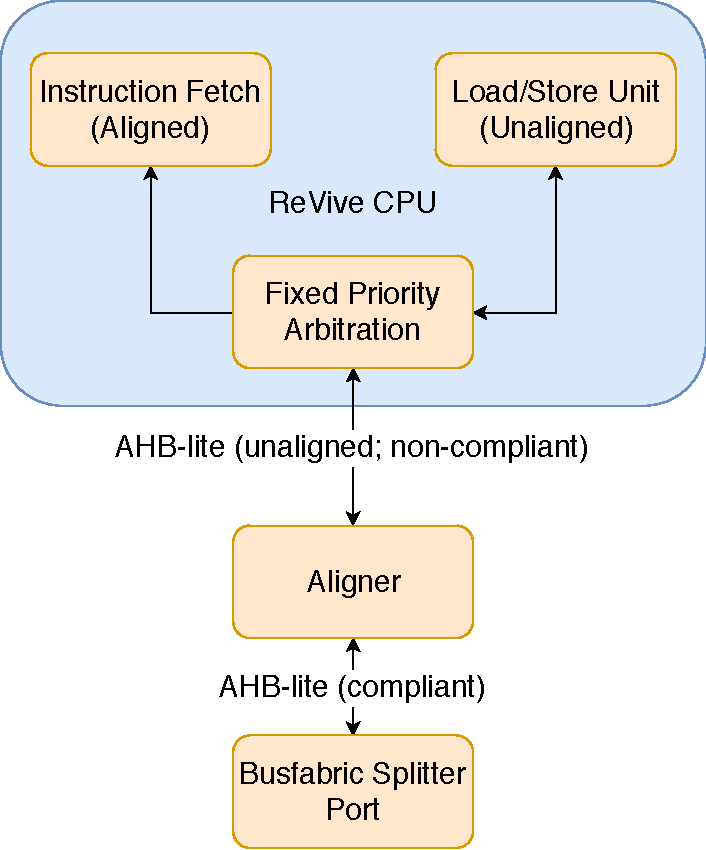
\includegraphics[width=0.4\textwidth]{diagrams/unaligned_accesses.pdf}
\end{figure}

\subsection{Interrupts}

ReVive has a single interrupt, implemented using the early jump hardware (\texttt{D}-triggered jumps). Upon raising of the interrrupt flag, the processor will abruptly jump to a predefined location (current plan is just to have this as a module parameter -- TODO). No state is saved on interrupt entry, except for the link register and the \texttt{PC}; the link register is overwritten with a magic value of \texttt{0xffffffff}, and a \texttt{jalr} to this address (most likely a \texttt{ret}) will trigger a jump back to the saved \texttt{PC}, and restoration of the stashed link register. This return is handled by the mispredict recovery hardware: \texttt{M} will see the magic jump value, initiating a jump to \texttt{PC} and swapping the stashed link register into the pipeline result register (making it visible to the bypass network).

It's up to the ISR to save any registers it uses. This may be a simple shell handler which saves the registers (caller- and callee-saved!) before dispatching out to a C function for each interrupt source. However, \textit{extremely} fast ISRs (2 cycle entry, 4 cycle exit) can be written by saving only those registers actually used.

Note that this model requires the stack pointer to be valid at all times. Software must set the stack pointer before unmasking interrupts in the external interrupt controller.

\subsection{Possible Performance Gains}

This section lists ideas of potential improvements which are waiting for synthesis + timing reports before I make a decision, or waiting for a decent regression test suite and working processor before I make complex changes.

\begin{itemize}
	\item The load/store address is generated by the ALU, which needs to mux its inputs and its operation. However, the inputs will always be rd1 and imm, and the operation is always add, so consider a hardwired adder to improve AHB timing.
	\item There is a large amount of muxing required at the end of the AHB data phase in \texttt{F}. It may be possible to move some of this muxing over the cycle boundary into \texttt{D}.
	\begin{itemize}
		\item \texttt{F} needs to look at the \texttt{CIR}, but \texttt{D} creating the \texttt{CIR} in-cycle will not affect \texttt{F}'s timing, because this will be in parallel with the AHB data phase.
		\item However, this may affect \texttt{W}'s address-phase timing, as \texttt{D}'s instruction size is used in fetch flow control.
	\end{itemize}
\end{itemize}

\section{Bus Fabric and Memory Subsystem}

Bus fabric is digital plumbing. A master, such as a processor, performs a read or write on some address; the bus fabric routes the transaction to the correct slave device, and routes the response back. FPGABoy implements two bus fabric standards:

\begin{itemize}
\item AMBA 3 AHB-lite connects masters to high-performance devices such as SRAM controllers
\item AMBA 3 APB connects to simple devices such as a UART
\end{itemize}

Figure \ref{diagram:crossbar_structure} shows the structure of the AHB-lite crossbar (\texttt{ahbl\_crossbar.v}). The crossbar is shown in context in figure \ref{diagram:system_arch}. An independent AHB-lite datapath connects each of $m$ masters to each of $n$ slaves. One master can address one slave at a time, and one slave can be in data-phase with one master at a time; subject to these constraints, up to $\min(m,n)$ independent transfers can take place in a single machine clock cycle.

Some claim AHB-lite does not "support" multi-master arbitration. These people lack imagination: motorbikes do not "support" wheelies by design, but are excellent at it.

\begin{figure}[!htb]
\centering
\caption{Module-level structure of AHB-lite crossbar} 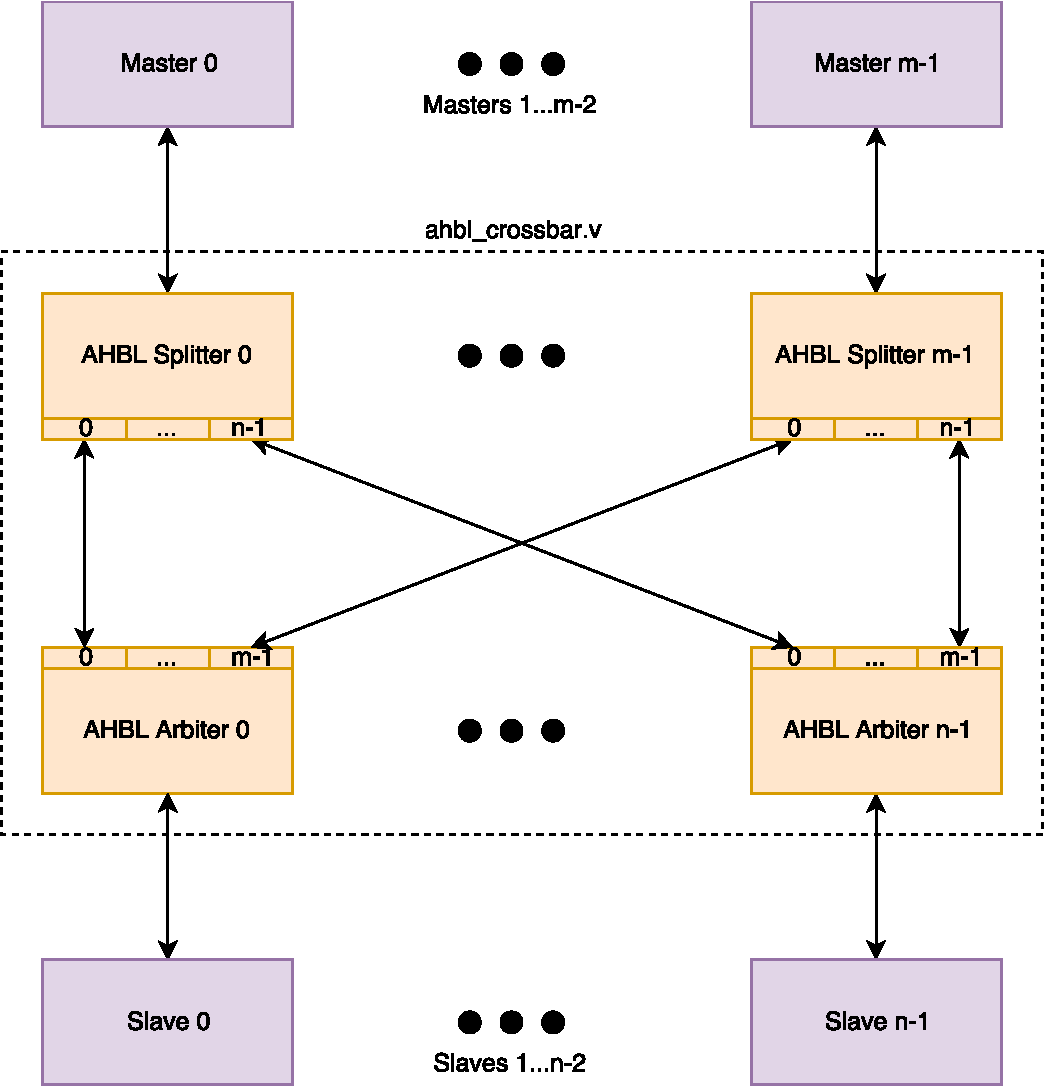
\includegraphics[width=0.6\textwidth]{diagrams/crossbar_structure.pdf}
\label{diagram:crossbar_structure}
\end{figure}

Each master is under the illusion that it is the only master in the system, but that slaves sometimes take longer to respond. During this waiting period, the slave may actually have fielded multiple transactions from higher-priority masters; this interaction handled by the slave's AHB-lite arbiter, and is transparent to the masters.

One of the crossbar's slave ports is attached to an AHBL-APB bridge. This bridge appears as a slave to the AHB portion of the bus fabric, and as a master to the APB portion. There are three main benefits to this scheme:

\begin{itemize}
	\item APB is fundamentally simpler
	\begin{itemize}
		\item This keeps peripheral gate count down
		\item The peripherals on the APB bus do not need the full AHB-lite bandwidth anyway
	\end{itemize}
	\item Fewer AHB-lite slaves
	\begin{itemize}
		\item There is a nonlinear area scaling associated with adding slaves to the AHB-lite fabric
		\item This would also add extra gate delays to a fairly critical data path
	\end{itemize}
	\item One APB master
	\begin{itemize}
		\item AHB-lite masters get arbitrated down to one inside the AHB-lite crossbar. APB slaves do not care who is addressing them.
		\item Different masters accessing different APB slaves will have to queue to use the bridge, even though they could theoretically proceed simultaneously
		\item However, area/complexity vs performance tradeoff is more than worth it for slow peripherals
		\item Multi-master APB is easy to implement, but never used in practice, due to the above tradeoff
	\end{itemize}
\end{itemize}

The splitter and arbiter modules in the AHB-lite crossbar can also be used on their own. Arbitrary multi-layer busfabric topologies should be possible with these two components.

\subsection{AHB-lite Primer}

For a full understanding of the bus standard used by FPGABoy, read through ARM's AMBA 3 AHB-lite spec. This document is mirrored in the \texttt{reference} folder in the GitHub repository, and gives a clear and comprehensive breakdown of AHB-lite. However, if you are feeling brave, the following overview should provide sufficient understanding of the standard to read through the Verilog.

AHB-lite is an asymmetric bus standard: masters assert transactions onto the bus, and slaves assert responses. Each transaction can be either a read or a write. The standard requires all transactions to be naturally aligned, i.e. the modulo of address and transfer size is zero. This is in tension with the RISC-V ISA which allows any transaction to have byte-alignment, so the load-store logic in the CPU may translate load/store instructions into multiple AHB-lite transactions.

AHB-lite has separate data paths for read and write. This reflects a move away from tristate logic in ASIC bus designs, and a lack of tristate logic in FPGAs.

AHB-lite transactions take place in two phases, named the address phase and the data phase. During the address phase, the master asserts signals which control the nature of the transfer, such as the address, whether the transfer is a read or write, protection/permission information, the width of the data, and so on. During the data phase, data is asserted on either the read or write data bus (\texttt{hrdata} and \texttt{hwdata}), but not both.

The central conceit of AHB-lite is that these two phases are \textit{pipelined}. Whilst the master is asserting or accepting data for an earlier transaction (currently in data phase), it concurrently asserts address and control information for a later transaction (currently in address phase). As is generally the case with pipelining, the goal is to enable higher clock frequencies with undiminished work-per-clock.

\begin{figure}[H]
\centering
\caption{A simple AHB-lite example}
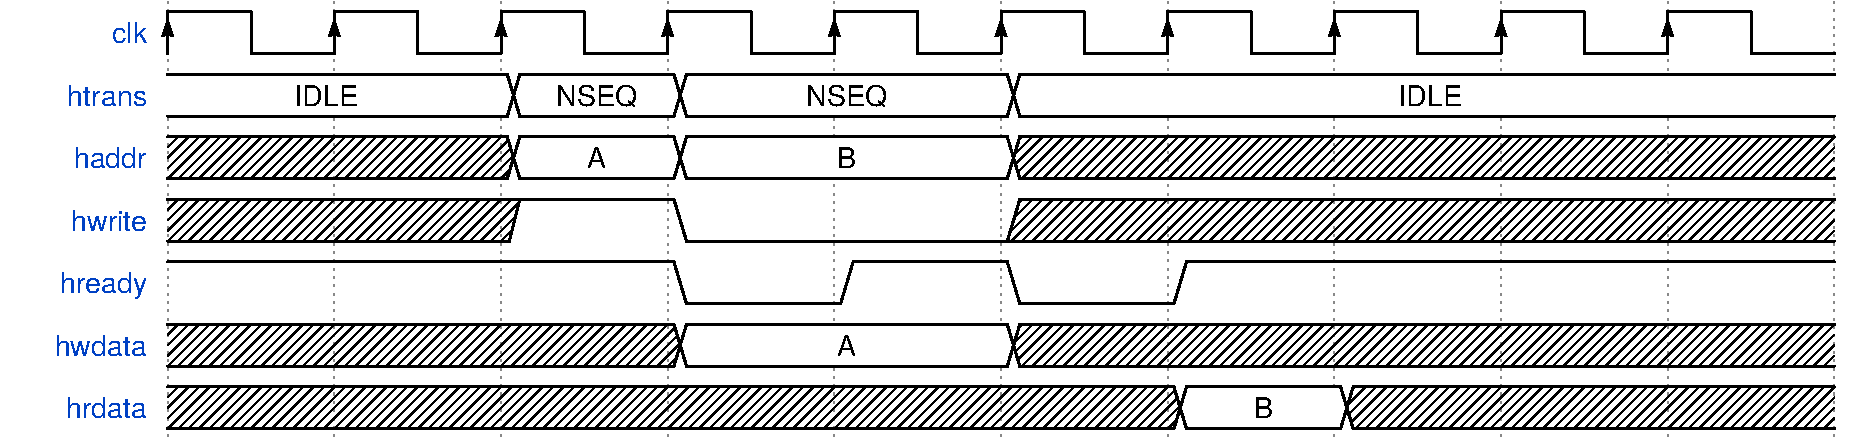
\includegraphics[width=0.9\textwidth]{waves/ahbl_basic.pdf}
\label{diagram:ahbl_basic}
\end{figure}

In figure \ref{diagram:ahbl_basic}, a master carries out two AHB-lite transactions: a write to address A, followed by a read from address B. Only a subset of AHB-lite signals are shown on the diagram.

The first three signals -- \texttt{htrans}, \texttt{haddr}, and \texttt{hwrite} -- are address phase, driven by the master; the others are data phase. \texttt{htrans} indicates the type of transaction the master next wishes to perform; allowed values are \texttt{IDLE}, \texttt{NSEQ} (non-sequential), \texttt{SEQ} and BUSY. The masters on FPGABoy only use \texttt{IDLE} and \texttt{NSEQ}. \texttt{hwrite} indicates the direction of the transaction, and \texttt{addr} the address (which is used for slave selection based on system memory map, and local address mapping inside of slaves).

\texttt{hready} signifies the end of the current data phase. As a result, the current address-phase transaction proceeds into data phase. Each slave has a signal called \texttt{hreadyout}, indicating that \textit{it} is ready, and the bus fabric selects the \texttt{hreadyout} of the current data-phase slave to be the global \texttt{hready}.

Initially, the bus is at rest. The master is asserting \texttt{IDLE} transactions. An \texttt{IDLE} data phase always completes in a single cycle. Therefore, the address phase for the first transaction -- write to address A -- also completes in a single cycle. When \texttt{htrans} is \texttt{IDLE}, the address-phase signals shown here are unimportant.

This slave needs two cycles to perform each data phase; perhaps it is an SRAM capable of running only at half the system clock speed. Therefore, \texttt{hready} is low for one cycle, and high for the second (last) cycle. The master drives \texttt{hwdata} for the duration of A's data phase, and waits for the slave to signal completion.

After 2 cycles, the data phase for address A completes. This is also the end of B's address phase. The data on \texttt{hrdata} is considered \textit{invalid} until the slave signals \texttt{hready}. During B's data phase, the master signals \texttt{IDLE}, as it has no further transactions to carry out after the read from B.

\subsection{Multi-Master Operation}

In a single-master busfabric, \texttt{hready} is a global signal, which causes the entire AHB-lite state machine (masters, slaves, fabric, the lot) to advance. Where multiple masters are concerned, \texttt{hready} is more subtle; in one respect, it is a per-master stall signal. In any case, \texttt{hready} is the most interesting and important wire on an AHB-lite bus. Consider figure \ref{diagram:ahbl_mm_simult1}, where two masters attempt to access a single slave simultaneously. Assume that master 0 always wins address-phase arbitration:

\begin{figure}[H]
\centering
\caption{Two masters access one slave.}
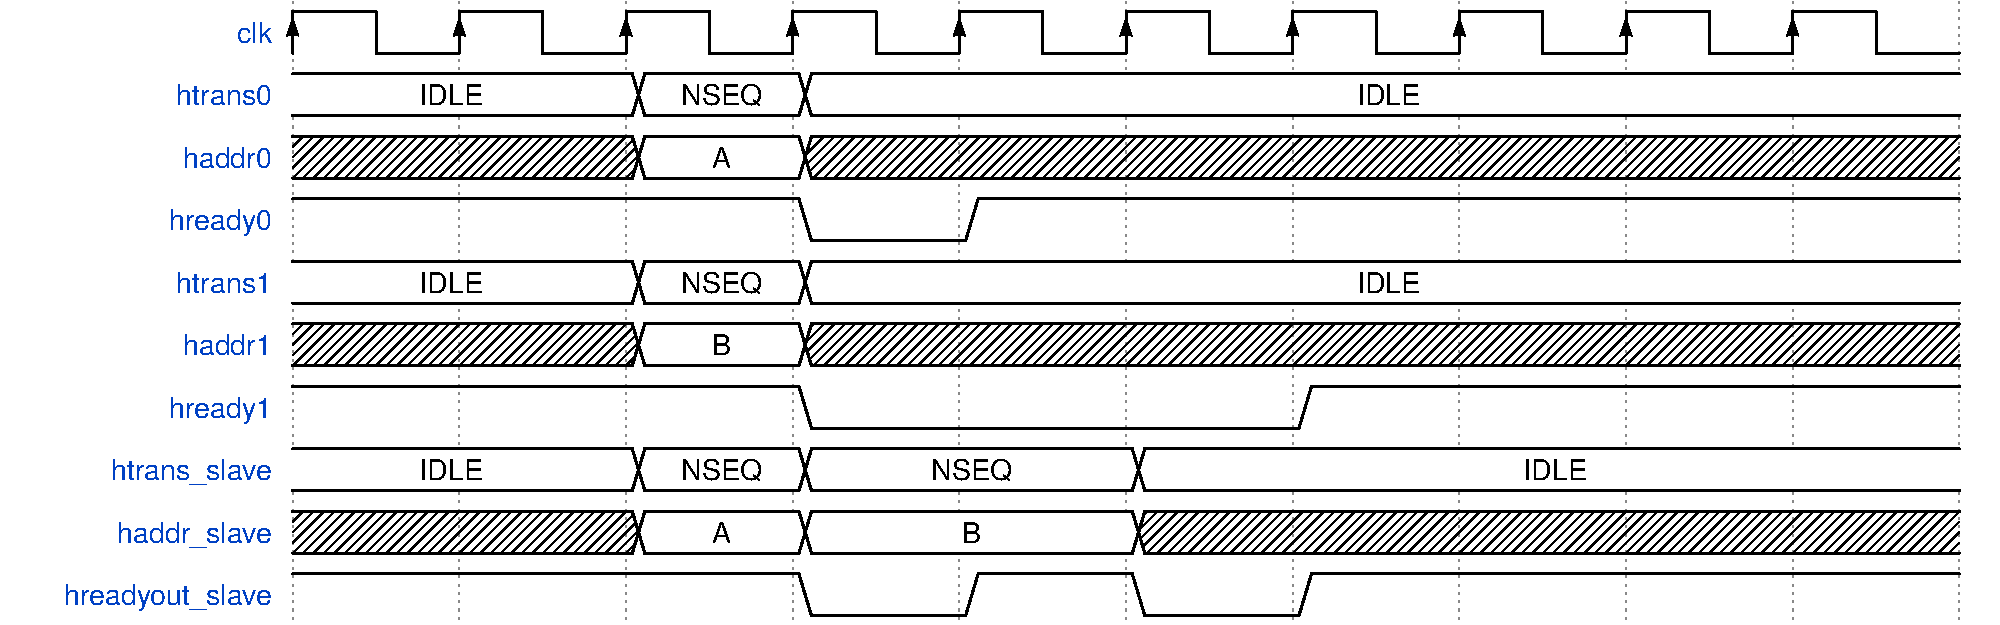
\includegraphics[width=0.9\textwidth]{waves/ahbl_mm_simult1.pdf}
\label{diagram:ahbl_mm_simult1}
\end{figure}

Again, we assume the slave requires 2 cycles to complete each data phase.

If we look at each master's trace, there is no indication at all that there is more than one master in the system: they present an address, and subsequently the transaction completes. Likewise, the slave neither knows nor cares that there are multiple masters: it simply carries out transactions according to the address-phase signals it sees. All of the smoke, mirrors and machinery are inside of the arbiter.

One odd feature of this trace is that, when the slave sees the address B, no master is asserting this address.

\begin{enumerate}
	\item Initially, both masters assert \texttt{IDLE}; \texttt{IDLE} data phases complete in one cycle
	\item \texttt{IDLE} data phases are concurrent with A, B address phases, so these \textit{also} complete immediately
	\item From the master 1's point of view, transaction B proceeds immediately to data phase.
	\item From both the master 0's and the slave's point of view, transaction A proceeds immediately to data phase
	\item Whilst the slave is in data phase for A, it is simultaneously in address phase for B
	\item When A data phase completes, master 0 is signaled, and B proceeds to data phase at the slave
	\item When B data phase completes, master 1 is signaled
\end{enumerate}

More concisely put, the first clock cycle of a given transaction's data phase may differ between the slave and master, but the \textit{last} cycle of that data phase is always the same clock cycle. This is a strong enough guarantee for correct operation.

Based on this discussion, the AHB-lite arbiters need the facility to buffer one address-phase request, per master. A buffered request will be applied before any new requests from that master, but after any higher-priority requests. There is a nonzero hardware cost to this buffering, but there are clear engineering benefits to keeping this complexity confined to the arbiters, as they are the only component in the busfabric which is explicitly "multi master".

\begin{figure}[H]
\centering
\caption{Two masters access one slave, with low-priority back-to-back}
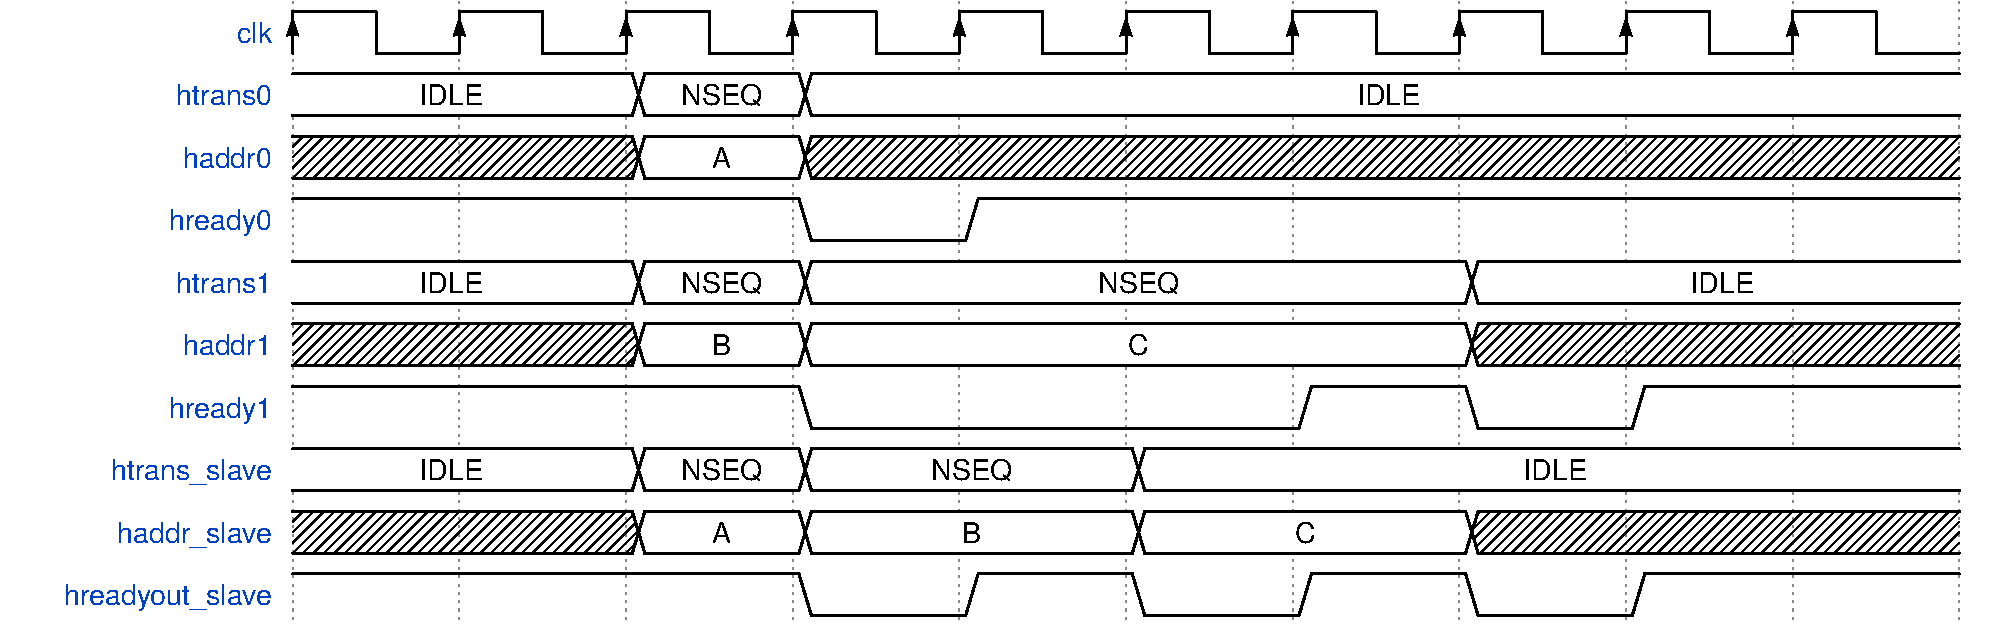
\includegraphics[width=0.9\textwidth]{waves/ahbl_mm_simult2.pdf}
\label{diagram:ahbl_mm_simult2}
\end{figure}

Figure \ref{diagram:ahbl_mm_simult2} shows the same sequence of events as figure \ref{diagram:ahbl_mm_simult1}, except master 0 now performs two back-to-back transactions. Once B's address phase completes, the arbiter's request buffer is cleared, and the C request passes transparently through the arbiter to the slave. Again, the only indication to master 1 of any master 0 activity is increased latency.

There is a different case which requires the arbiter's request buffer, shown in figure \ref{diagram:ahbl_mm_simult3}.

\begin{figure}[H]
\centering
\caption{Simultaneous request buffer writes}
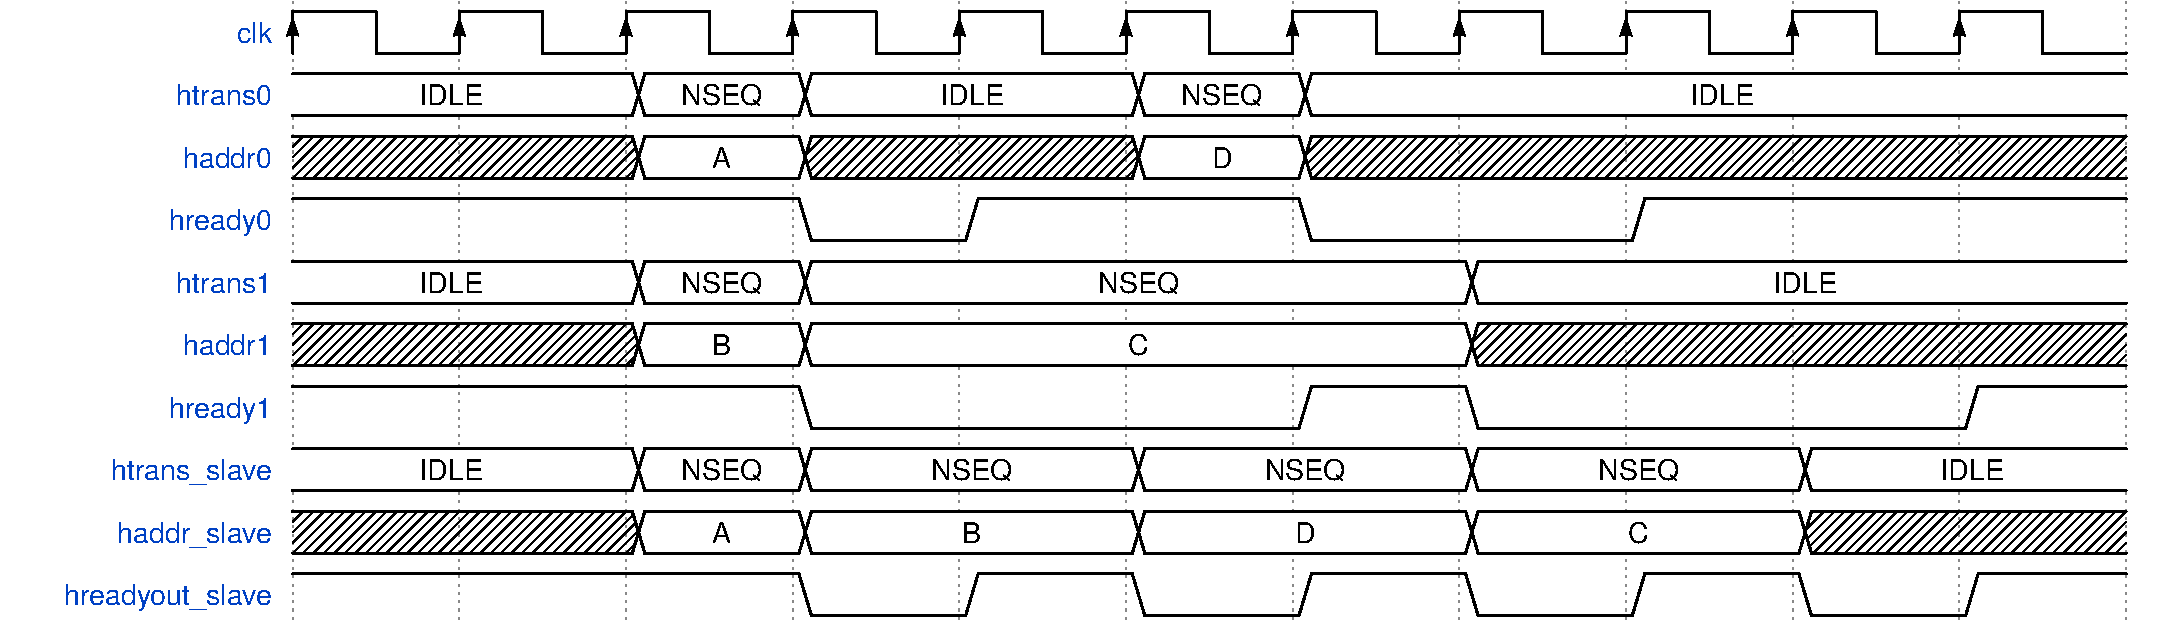
\includegraphics[width=0.9\textwidth]{waves/ahbl_mm_simult3.pdf}
\label{diagram:ahbl_mm_simult3}
\end{figure}

At the instant where D address phase is asserted, \texttt{hready0} is high, because master 0 previously asserted an \texttt{IDLE} transfer. However, the slave is not ready. In this case, the arbiter needs to buffer master 0's request, even though it is the highest-priority master. The buffered request is cleared once its slave address phase completes, as usual.

There is one final case, for two masters accessing one slave, which is worth being aware of (figure \ref{diagram:ahbl_mm_latearrival}).

\begin{figure}[H]
\centering
\caption{High-priority late arrival}
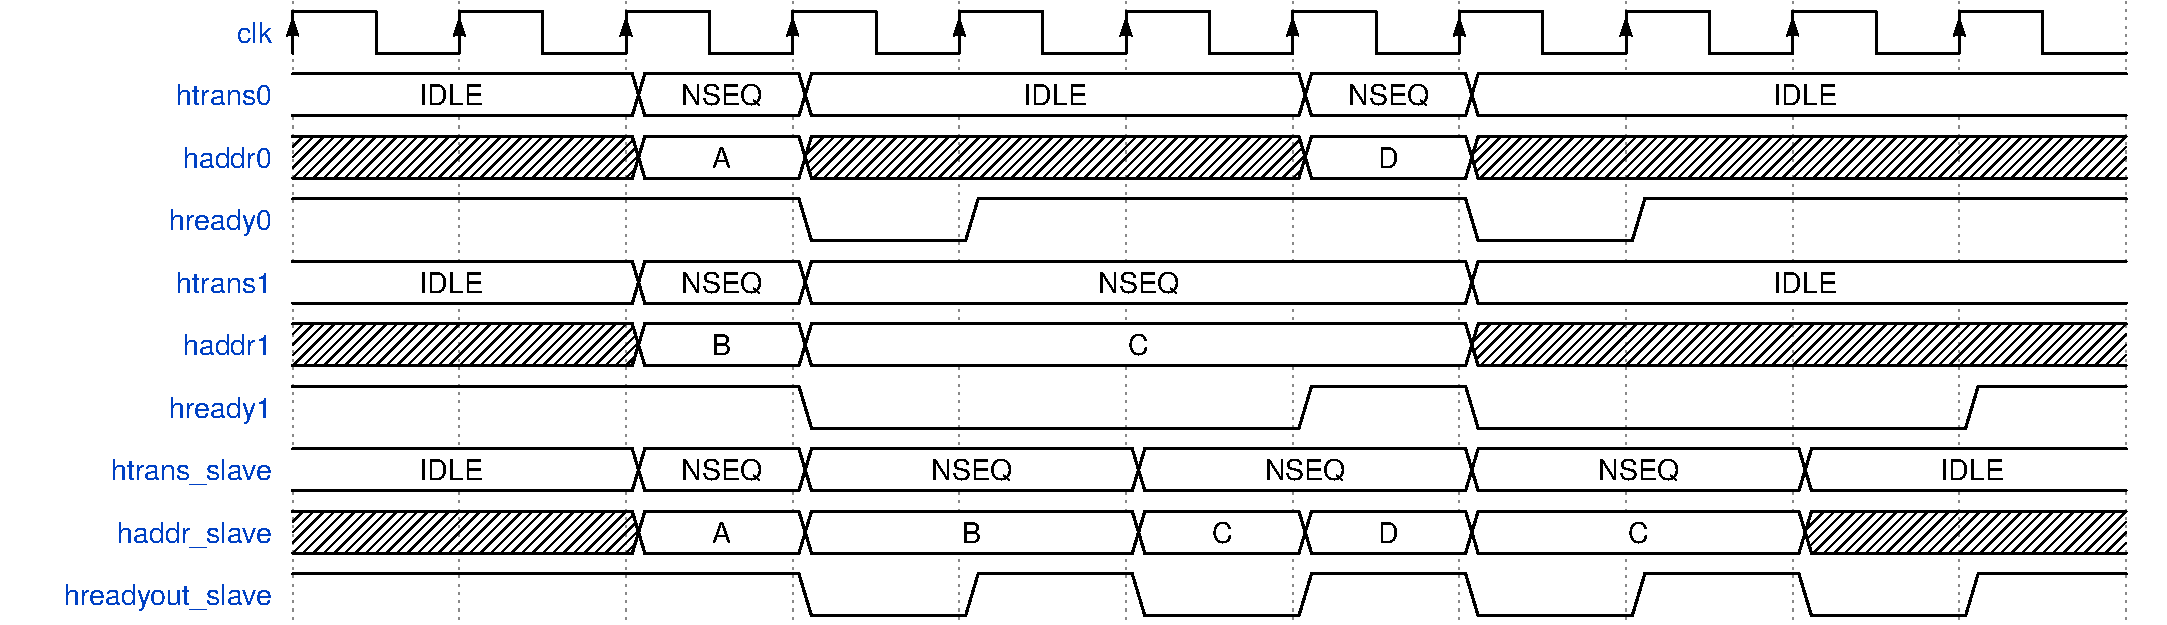
\includegraphics[width=0.9\textwidth]{waves/ahbl_mm_latearrival.pdf}
\label{diagram:ahbl_mm_latearrival}
\end{figure}

Whilst \texttt{hreadyout} is low, the C address briefly appears on the slave bus, before being replaced by the higher-priority D request. \textbf{This is a departure from the AHB-lite standard}, which stipulates the address must be constant during this time. This is deliberate, and could easily be amended. Slaves are generally insensitive to address-phase request during this time (as there is no performance benefit to latching AP before \texttt{hreadyout}, due to the way the bus operates), and this avoids a priority inversion, reducing average latency for higher-priority masters. If you find something that this breaks, write me an angry email! I would be genuinely curious to see such a slave.

\section{Graphics Pipeline}

The graphics pipeline is still at the whiteboard stage, and its final form will depend on how many gates are left over when the rest of the system is finished. However, it will look something like the following (potentially without the affine transform blocks):

\begin{figure}[!htb]
\centering
\caption{Block-level diagram of graphics pipeline}
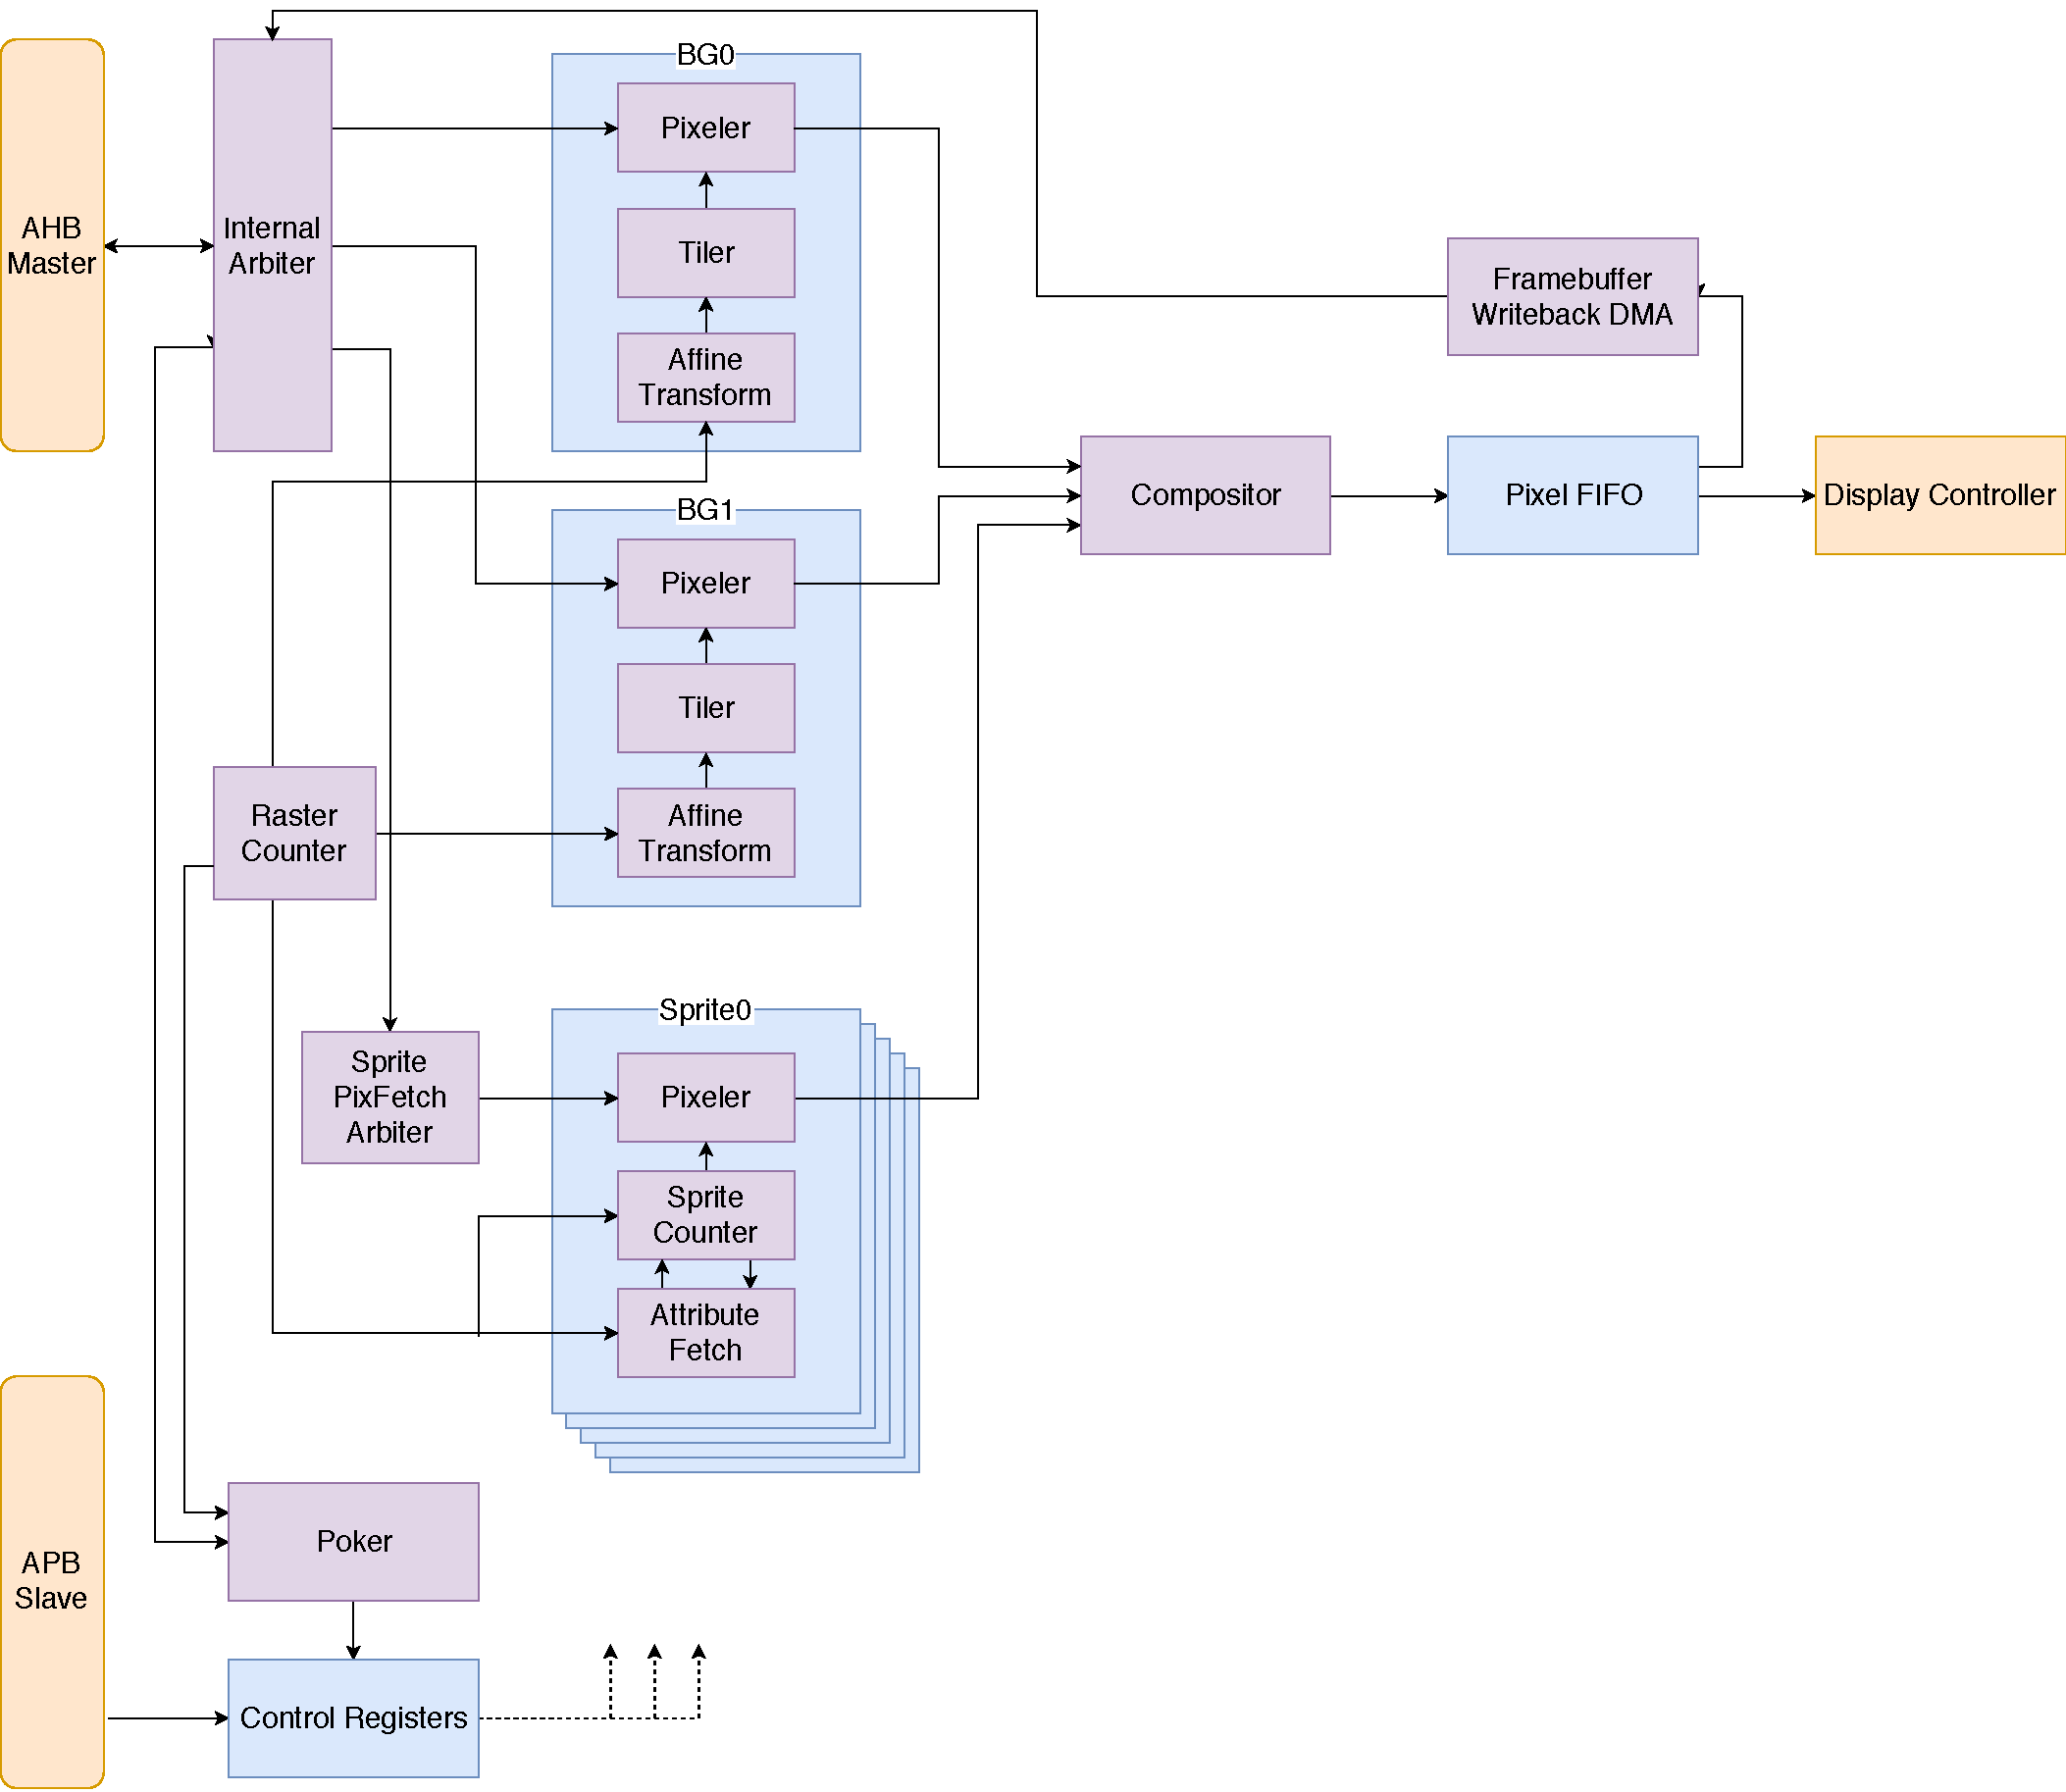
\includegraphics[width=0.9\textwidth]{diagrams/graphics.pdf}
\end{figure}

The poker is a simple raster-synchronised coprocessor which can poke control registers at precise points during a scanline; similar to the Copper on an Amiga. This would be particularly powerful in conjunction with background affine transform!

\end{document}